\begin{frame}\begin{center}
\LARGE\textbf{Setup}
\end{center}\end{frame}



\begin{frame}
\textbf{Setup}
\begin{itemize}\setlength\itemsep{1em}
\item Normal linear-in-parameters version of the generalized Roy model.
\end{itemize}
\begin{align*}
\text{Potential Outcomes} &\qquad \text{Cost} \\
Y_1 = \beta_1 X + U_1      &\qquad C = \gamma Z + U_C \\
Y_0 = \beta_0 X + U_0      &\qquad \\
    & \\
\text{Observed Outcomes}  &\qquad \text{Choice} \\
Y = D Y_1 + (1 - D)Y_0 &\qquad S = Y_1 - Y_0 - C \\
                       &\qquad D = \mathrm{I}[S > 0] \\
\end{align*}
\end{frame}

\begin{frame}\begin{center}
\LARGE\textbf{Features}
\end{center}\end{frame}

\begin{frame}
\textbf{Features}
\begin{itemize}\setlength\itemsep{1em}
\item \textit{grmpy} is currently capable of the following features:
\begin{itemize}\setlength\itemsep{1em}
  \item Simulating a dataset based on your own specifications.
  \item Providing some useful information about the simulated dataset for instance:
    \begin{itemize}\setlength\itemsep{1em}
    \item Distributional outcome characteristics
    \item ATE, TT, TUT
    \item MTE by ventile
    \end{itemize}
  \item Estimating the coefficients of interest given a dataset (of a specific form).
\end{itemize}
\end{itemize}

\end{frame}

\begin{frame}
\textbf{Install the package}
\begin{itemize}\setlength\itemsep{1em}
\item OS, Linux : Use the pip install manager (\textit{pip install grmpy}) or download the package via \href{https://github.com/grmToolbox/grmpy}{GitHub} and install it manually.
\item Windows:  The same procedure as for Linux, OS but you have to verify that the numpy package is already installed on your machine.
\end{itemize}
\end{frame}

\begin{frame}
\textbf{Initialization file}
\begin{itemize}\setlength\itemsep{1em}
\item The initialization file provides the user with the opportunity to specify all parameters of his/her model, for instance:\medskip
  \begin{itemize}\setlength\itemsep{1em}
  \item Simulation parameters (number of observations, name of the output files)
  \item Estimation parameters (optimization algorithm, start values)
  \item Optimization parameters
  \item Coefficients and covariance parameters, dummy variables...
  \end{itemize}
\item \href{../shared/04_grmpy_tutorial/application/tutorial.grmpy.ini}{Example}
\item for a detailed explanation see: \href{http://grmpy.readthedocs.io/en/latest/tutorial.html}{\textit{grmpy}-documentation}
\end{itemize}
\end{frame}

\begin{frame}
\textbf{Simulation}
\begin{itemize}\setlength\itemsep{1em}
\item \textit{grmpy.simulate():}\medskip
\begin{itemize}\setlength\itemsep{1em}
\item Input: path of the initialization file.
\item The function returns a data frame based on your specifications and different output files.
\begin{itemize}\setlength\itemsep{1em}
\item The data set as a pickle and a txt file.
\item An \href{../04_grmpy_tutorial_notebook/examples/data.grmpy.info}{Info file} that provides the distributional characteristics of the data as well as information about the different treatment effects.
\end{itemize}

\end{itemize}
\end{itemize}
\end{frame}

\begin{frame}
\textbf{Estimation}
\begin{itemize}\setlength\itemsep{1em}
\item \textit{grmpy.estimate():}\medskip
  \begin{itemize}\setlength\itemsep{1em}
  \item Input: path of the initialization file.
  \item At the moment the estimation process is only capable of two different optimization algorithms:
    \begin{itemize}\setlength\itemsep{1em}
    \item Broyden Fletcher Goldfarb Shanno (BFGS) algorithm
    \item  Powell's conjugate direction method
\end{itemize}
\end{itemize}
\end{itemize}

\end{frame}

\begin{frame}
\begin{itemize}\setlength\itemsep{1em}
\item There are two different options for the start values that could be set in the initialization file:\medskip
  \begin{itemize}\setlength\itemsep{1em}
  \item \textit{init:} The estimation process uses the coefficient values specified in the initialization file as the start values for the estimation process.
  \item \textit{auto:} The start values are determined via a simple OLS followed by a Probit regression for the choice indicator.
  \end{itemize}
  \item The estimation results are printed to an \href{../04_grmpy_tutorial_notebook/examples/est.grmpy.info}{output file}
\end{itemize}
\end{frame}

\begin{frame}
\textbf{Test battery}
\begin{itemize}\setlength\itemsep{1em}
\item We also provide a test battery that includes several tests to ensure that the processes perform as intended.\medskip
\begin{itemize}\setlength\itemsep{1em}
\item Property-based testing
\item Reliability testing
\item Regression testing
\end{itemize}
\end{itemize}
\end{frame}

\begin{frame}
	\textbf{What's yet to come?}
	\begin{itemize}
		\item Partial replication of \citeA{Carneiro.2011} (very soon!)
		\item Addition of marginal surplus and marginal cost parameters
		\item Implementation of polynomial and local instrumental variable estimation
		\item Exploration of alternative optimization algorithms to address large estimation tasks
	\end{itemize}
\end{frame}

\begin{frame}\begin{center}
\LARGE\textbf{Application Example}
\end{center}\end{frame}


\begin{frame}\begin{center}
\LARGE\textbf{Additional Information}
\end{center}\end{frame}

\begin{frame}
\textbf{Online documentation}
\begin{figure}
  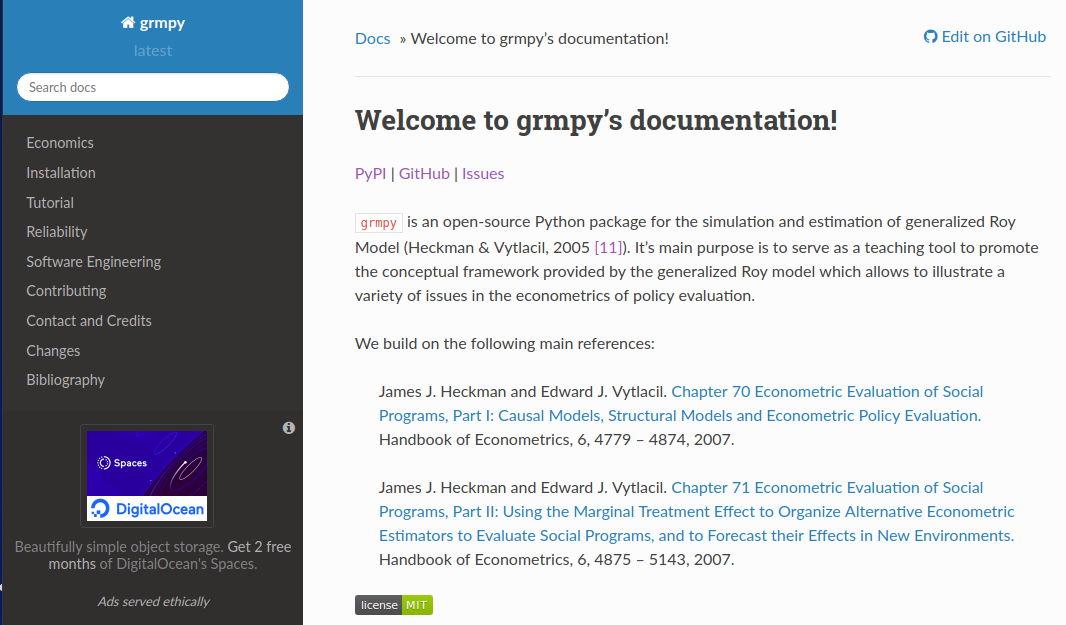
\includegraphics[scale=0.2]{../04_grmpy_tutorial_notebook/docu.png}
\end{figure}

\end{frame}
